\documentclass[conference]{IEEEtran}
\IEEEoverridecommandlockouts
\usepackage{cite}
\usepackage{amsmath,amssymb,amsfonts}
\usepackage{algorithmic}
\usepackage{graphicx}
\usepackage{textcomp}
\usepackage{xcolor}
\usepackage{booktabs}
\usepackage[hidelinks]{hyperref}
\usepackage{tikz}
\usetikzlibrary{shapes.geometric, arrows.meta, positioning}
\graphicspath{{./figures/}}

\def\BibTeX{{\rm B\kern-.05em{\sc i\kern-.025em b}\kern-.08em
    T\kern-.1667em\lower.7ex\hbox{E}\kern-.125emX}}

\begin{document}

\title{Face Recognition Based Smart Attendance System Using MTCNN and FaceNet}

\author{
\IEEEauthorblockN{Deepak Singh}
\IEEEauthorblockA{
    \textit{Department of Computer Science and Engineering}\\
    \textit{Indian Institute of Information Technology Surat}\\
    Surat, Gujarat, India\\
    ui23cs17@iiitsurat.ac.in
}
\and
\IEEEauthorblockN{Harsh Khulbe}
\IEEEauthorblockA{
    \textit{Department of Computer Science and Engineering}\\
    \textit{Indian Institute of Information Technology Surat}\\
    Surat, Gujarat, India\\
    ui23cs26@iiitsurat.ac.in
}
}

\maketitle

% -------------------------------------------------------------------
\begin{abstract}
Traditional manual attendance systems in educational institutions are
time-consuming, error-prone, and susceptible to proxy attendance. This
paper proposes a Smart Attendance System that automates the entire
attendance process using computer-vision and deep-learning techniques.
The system employs the Multi-task Cascaded Convolutional Network (MTCNN)
for robust face detection, and a pre-trained FaceNet Convolutional Neural
Network (CNN) model for generating high-dimensional facial embeddings.
During enrollment, short video clips of each student are recorded; frames
are extracted, faces detected, aligned to a canonical 160$\times$160 size,
and embedded into a 512-dimensional feature vector. These embeddings are
stored in a persistent database. At recognition time, a group photograph
is processed by the same pipeline, and identified faces are matched to
enrolled students via Euclidean distance with a configurable threshold.
Matched identities are automatically logged to a dated CSV attendance
register. Experimental results demonstrate high recognition accuracy and
robustness to moderate illumination and pose variation, making the system
a practical drop-in replacement for manual roll-calls.
\end{abstract}

\begin{IEEEkeywords}
face recognition, MTCNN, FaceNet, CNN, attendance system, OpenCV,
facial embeddings, deep learning
\end{IEEEkeywords}

% -------------------------------------------------------------------
\section{Introduction}

Attendance tracking is a fundamental administrative task in schools,
colleges, and corporate settings. Conventional methods---paper registers,
card-swipe systems, and manual roll-calls---are slow, labour-intensive,
and vulnerable to buddy-punching (proxy attendance). The rapid maturation
of deep learning and computer vision offers an opportunity to fully
automate this process in a non-intrusive manner.

Convolutional Neural Networks (CNNs) have revolutionised face analysis
since the seminal work of LeCun \emph{et al.} \cite{b1}. Modern face
verification systems such as DeepFace \cite{b2} and FaceNet \cite{b3}
achieve near-human accuracy by mapping face images to compact
Euclidean-space embeddings, where intra-personal variation is small and
inter-personal variation is large. Combined with lightweight real-time
detectors such as MTCNN \cite{b4}, these techniques enable practical
end-to-end attendance pipelines that run on commodity hardware.

This paper presents a two-phase Smart Attendance System:
\begin{itemize}
    \item \textbf{Phase 1 -- Enrolment:} video-to-face-embedding
          database construction for each student.
    \item \textbf{Phase 2 -- Recognition:} group-image face detection,
          embedding extraction, nearest-neighbour matching, and
          automatic CSV logging.
\end{itemize}

The remainder of the paper is organised as follows. Section II surveys
related work. Section III describes the proposed system architecture.
Section IV details the implementation. Section V presents experimental
results, and Section VI concludes.

% -------------------------------------------------------------------
\section{Related Work}

Early automated attendance systems relied on eigenfaces \cite{b5} (PCA)
and Linear Discriminant Analysis (LDA), which perform poorly under
illumination changes and occlusion. The introduction of Local Binary
Patterns (LBP) \cite{b6} improved robustness but remained sensitive to
large pose variations.

Deep learning changed the landscape fundamentally. DeepFace \cite{b2}
used a nine-layer CNN trained on four million images to achieve
97.35\% accuracy on the Labeled Faces in the Wild (LFW) benchmark---comparable
to human performance. FaceNet \cite{b3} adopted a triplet-loss training
strategy and an Inception architecture to produce 128-dimensional
embeddings with state-of-the-art results. MTCNN \cite{b4} introduced a
cascaded three-stage detector (P-Net, R-Net, O-Net) that jointly detects
faces and five facial landmarks in a single forward pass, and has since
become the de facto detection front-end in attendance pipelines.

Arsenovic et al. \cite{b10} presented \emph{FaceTime}, one of the earliest
end-to-end deep-learning attendance systems, at the IEEE SISY 2017 conference.
Their architecture employed a cascaded CNN for face detection coupled with a
separate recognition network, achieving approximately 95\% recognition accuracy
in real-world classroom conditions. While the system demonstrated that deep
learning could replace traditional keypoint-based methods for attendance, the
authors acknowledged that scalability was constrained by a small, institution-specific
dataset and the computational cost of per-frame recognition on contemporary hardware.

Alhanaee et al. \cite{b11} investigated transfer learning as a strategy to
overcome the data-scarcity problem common in institutional settings. Published in
\emph{Procedia Computer Science} (2021), their study fine-tuned three well-known
pre-trained CNN architectures---AlexNet, GoogleNet, and SqueezeNet---on custom
student face datasets. AlexNet achieved validation accuracies of up to 100\% but
incurred the longest training time, while SqueezeNet offered a competitive
speed--accuracy trade-off due to its compact architecture. The work established
that transfer learning can yield very high accuracy even when training data are
limited, but it relies on an initial fine-tuning phase per deployment.

Kadam et al. \cite{b12} proposed a group-photo attendance system combining
MTCNN detection with a CNN-based recognition model backed by a MySQL database,
reported in 2025. The system achieved approximately 98\% accuracy with an average
end-to-end processing time of 2.3 seconds per group image, and demonstrated
robustness to moderate illumination variation---directly addressing classroom
conditions. Their use of a relational database for record management represents
a production-oriented design choice absent from most research prototypes.

The present work differs from these studies in three key respects: (1) it uses
the pre-trained FaceNet model to generate 512-dimensional embeddings, avoiding
the fine-tuning step required by transfer-learning approaches; (2) it replaces
database-backed storage with a lightweight pickle-serialised embedding dictionary,
simplifying deployment on edge hardware; and (3) vectorised NumPy nearest-neighbour
matching provides $O(N)$ complexity with C-level performance, making the pipeline
scalable without a dedicated GPU.

% -------------------------------------------------------------------
\section{System Architecture}

The proposed system is composed of two major phases, each implemented
as an independent, importable Python module.

\subsection{Phase 1: Dataset Creation and Enrolment}

\begin{enumerate}
    \item \textbf{Frame Extraction} -- Short enrollment video clips
          (5--10 s per student) are sampled at 2 fps using OpenCV's
          \texttt{VideoCapture} API, yielding 10--20 diverse frames
          per person.
    \item \textbf{Face Detection} -- MTCNN \cite{b4} localises every
          face in each frame, returning bounding-box coordinates.
          Detected regions are cropped to the bounding box.
    \item \textbf{Face Alignment} -- Each cropped face is resized to
          $160\times160$ pixels, the canonical input resolution of
          FaceNet, using bicubic interpolation.
    \item \textbf{Embedding Generation} -- The aligned face is passed
          through the pre-trained \texttt{keras-facenet} model,
          producing a 512-dimensional unit-norm embedding vector.
    \item \textbf{Database Construction} -- All per-person embeddings
          are serialised into a Python dictionary and persisted as a
          \texttt{.pkl} file (\texttt{embeddings.pkl}).
\end{enumerate}

The activity flow for Phase~1 is shown in Fig.~\ref{fig:act_phase1}.

\begin{figure}[htbp]
\centering
\resizebox{0.48\columnwidth}{!}{%
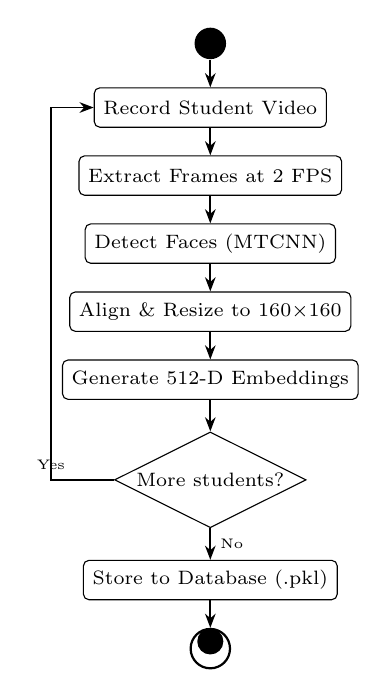
\begin{tikzpicture}[node distance=0.35cm,
    startstop/.style={circle, fill=black, minimum size=4mm},
    endnode/.style={circle, draw=black, thick, minimum size=5mm, inner sep=0pt},
    process/.style={rectangle, rounded corners=2pt, draw=black,
                    minimum width=2.8cm, minimum height=0.5cm,
                    text centered, font=\scriptsize},
    decision/.style={diamond, draw=black, aspect=2,
                     text centered, font=\scriptsize, inner sep=1pt},
    arrow/.style={-{Stealth[length=1.8mm]}, semithick}
]
\node (start) [startstop] {};
\node (rec)   [process, below=of start] {Record Student Video};
\node (ext)   [process, below=of rec]   {Extract Frames at 2 FPS};
\node (det)   [process, below=of ext]   {Detect Faces (MTCNN)};
\node (ali)   [process, below=of det]   {Align \& Resize to $160{\times}160$};
\node (emb)   [process, below=of ali]   {Generate 512-D Embeddings};
\node (dec)   [decision, below=0.4cm of emb] {More students?};
\node (store) [process, below=0.4cm of dec]  {Store to Database (.pkl)};
\node (endd)  [startstop, below=of store, minimum size=3mm] {};
\node (endring) [endnode, below=of store] {};

\draw [arrow] (start) -- (rec);
\draw [arrow] (rec)   -- (ext);
\draw [arrow] (ext)   -- (det);
\draw [arrow] (det)   -- (ali);
\draw [arrow] (ali)   -- (emb);
\draw [arrow] (emb)   -- (dec);
\draw [arrow] (dec)   -- node[right, font=\tiny]{No} (store);
\draw [arrow] (dec.west) -- ++(-0.8,0) node[above, font=\tiny]{Yes}
              |- (rec.west);
\draw [arrow] (store) -- (endring);
\end{tikzpicture}
}%
\caption{Activity diagram for Phase~1: Dataset creation and enrolment.}
\label{fig:act_phase1}
\end{figure}

\subsection{Phase 2: Attendance Recognition}

\begin{enumerate}
    \item \textbf{Group Image Input} -- One or more group photographs
          of the classroom are supplied.
    \item \textbf{Face Detection} -- MTCNN detects and crops all faces
          in the image, each resized to $160\times160$ px.
    \item \textbf{Embedding Extraction} -- FaceNet maps each cropped
          face to its 512-D embedding.
    \item \textbf{Nearest-Neighbour Matching} -- For every query
          embedding $\mathbf{e}_{q}$, the Euclidean distance to every
          stored embedding $\mathbf{e}_{i}$ is computed via a vectorised
          NumPy operation:
          \begin{equation}
              d_i = \|\mathbf{e}_q - \mathbf{e}_i\|_2
              \label{eq:euclid}
          \end{equation}
          If $\min(d_i) < \tau$ (threshold $\tau = 0.6$), the face is
          assigned to the corresponding identity; otherwise it is labelled
          \emph{Unknown}.
    \item \textbf{Attendance Logging} -- Recognised names are de-duplicated
          and appended to a date-stamped CSV file
          (\texttt{attendance\_YYYY-MM-DD.csv}) with columns
          \textit{Name}, \textit{Status}, and \textit{Time}.
    \item \textbf{Result Visualisation} -- Bounding boxes and name labels
          are drawn on the group image using OpenCV and displayed.
\end{enumerate}

The activity flow for Phase~2 is shown in Fig.~\ref{fig:act_phase2}.

\begin{figure}[htbp]
\centering
\resizebox{0.55\columnwidth}{!}{%
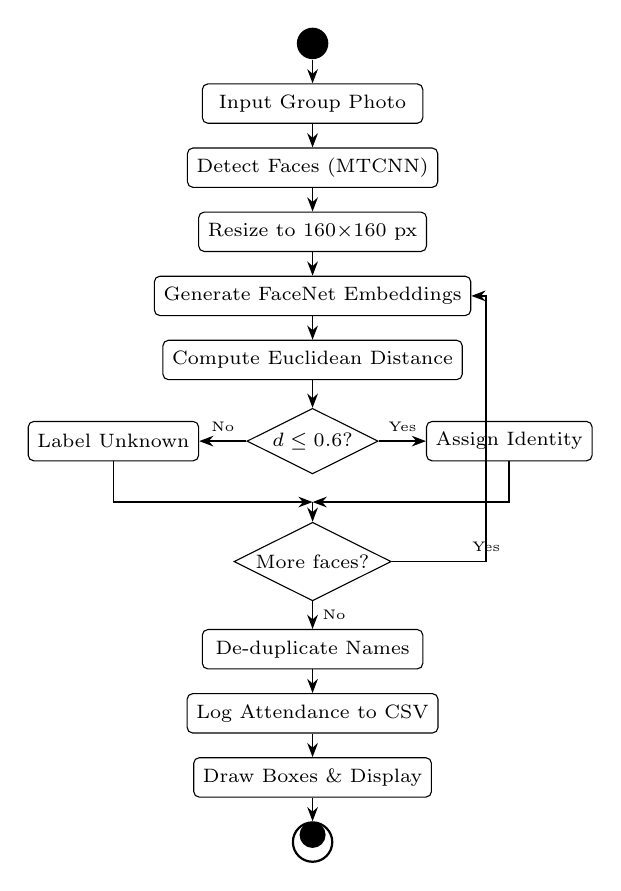
\begin{tikzpicture}[node distance=0.3cm,
    startstop/.style={circle, fill=black, minimum size=4mm},
    endnode/.style={circle, draw=black, thick, minimum size=5mm, inner sep=0pt},
    process/.style={rectangle, rounded corners=2pt, draw=black,
                    minimum width=2.8cm, minimum height=0.5cm,
                    text centered, font=\scriptsize},
    decision/.style={diamond, draw=black, aspect=2,
                     text centered, font=\scriptsize, inner sep=1pt},
    arrow/.style={-{Stealth[length=1.8mm]}, semithick}
]
\node (start) [startstop] {};
\node (inp)   [process, below=of start] {Input Group Photo};
\node (det)   [process, below=of inp]   {Detect Faces (MTCNN)};
\node (rsz)   [process, below=of det]   {Resize to $160{\times}160$ px};
\node (emb)   [process, below=of rsz]   {Generate FaceNet Embeddings};
\node (dist)  [process, below=of emb]   {Compute Euclidean Distance};
\node (dec1)  [decision, below=0.35cm of dist] {$d \leq 0.6$?};
\node (yes)   [process, right=0.6cm of dec1, minimum width=1.8cm] {Assign Identity};
\node (no)    [process, left=0.6cm of dec1, minimum width=1.8cm]  {Label Unknown};
\node (merge) [coordinate, below=0.35cm of dec1] {};
\node (dec2)  [decision, below=0.25cm of merge] {More faces?};
\node (dedup) [process, below=0.35cm of dec2]  {De-duplicate Names};
\node (csv)   [process, below=of dedup] {Log Attendance to CSV};
\node (draw)  [process, below=of csv]   {Draw Boxes \& Display};
\node (endd)  [startstop, below=of draw, minimum size=3mm] {};
\node (endring) [endnode, below=of draw] {};

\draw [arrow] (start) -- (inp);
\draw [arrow] (inp)   -- (det);
\draw [arrow] (det)   -- (rsz);
\draw [arrow] (rsz)   -- (emb);
\draw [arrow] (emb)   -- (dist);
\draw [arrow] (dist)  -- (dec1);
\draw [arrow] (dec1)  -- node[above, font=\tiny]{Yes} (yes);
\draw [arrow] (dec1)  -- node[above, font=\tiny]{No}  (no);
\draw [arrow] (yes.south) |- (merge);
\draw [arrow] (no.south)  |- (merge);
\draw [arrow] (merge) -- (dec2);
\draw [arrow] (dec2)  -- node[right, font=\tiny]{No} (dedup);
\draw [arrow] (dec2.east) -- ++(1.2,0) node[above, font=\tiny]{Yes}
              |- (emb.east);
\draw [arrow] (dedup) -- (csv);
\draw [arrow] (csv)   -- (draw);
\draw [arrow] (draw)  -- (endring);
\end{tikzpicture}
}%
\caption{Activity diagram for Phase~2: Attendance recognition and logging.}
\label{fig:act_phase2}
\end{figure}

The overall system class structure is shown in Fig.~\ref{fig:classdiag}.

\begin{figure*}[htbp]
\centering
\resizebox{0.95\textwidth}{!}{%
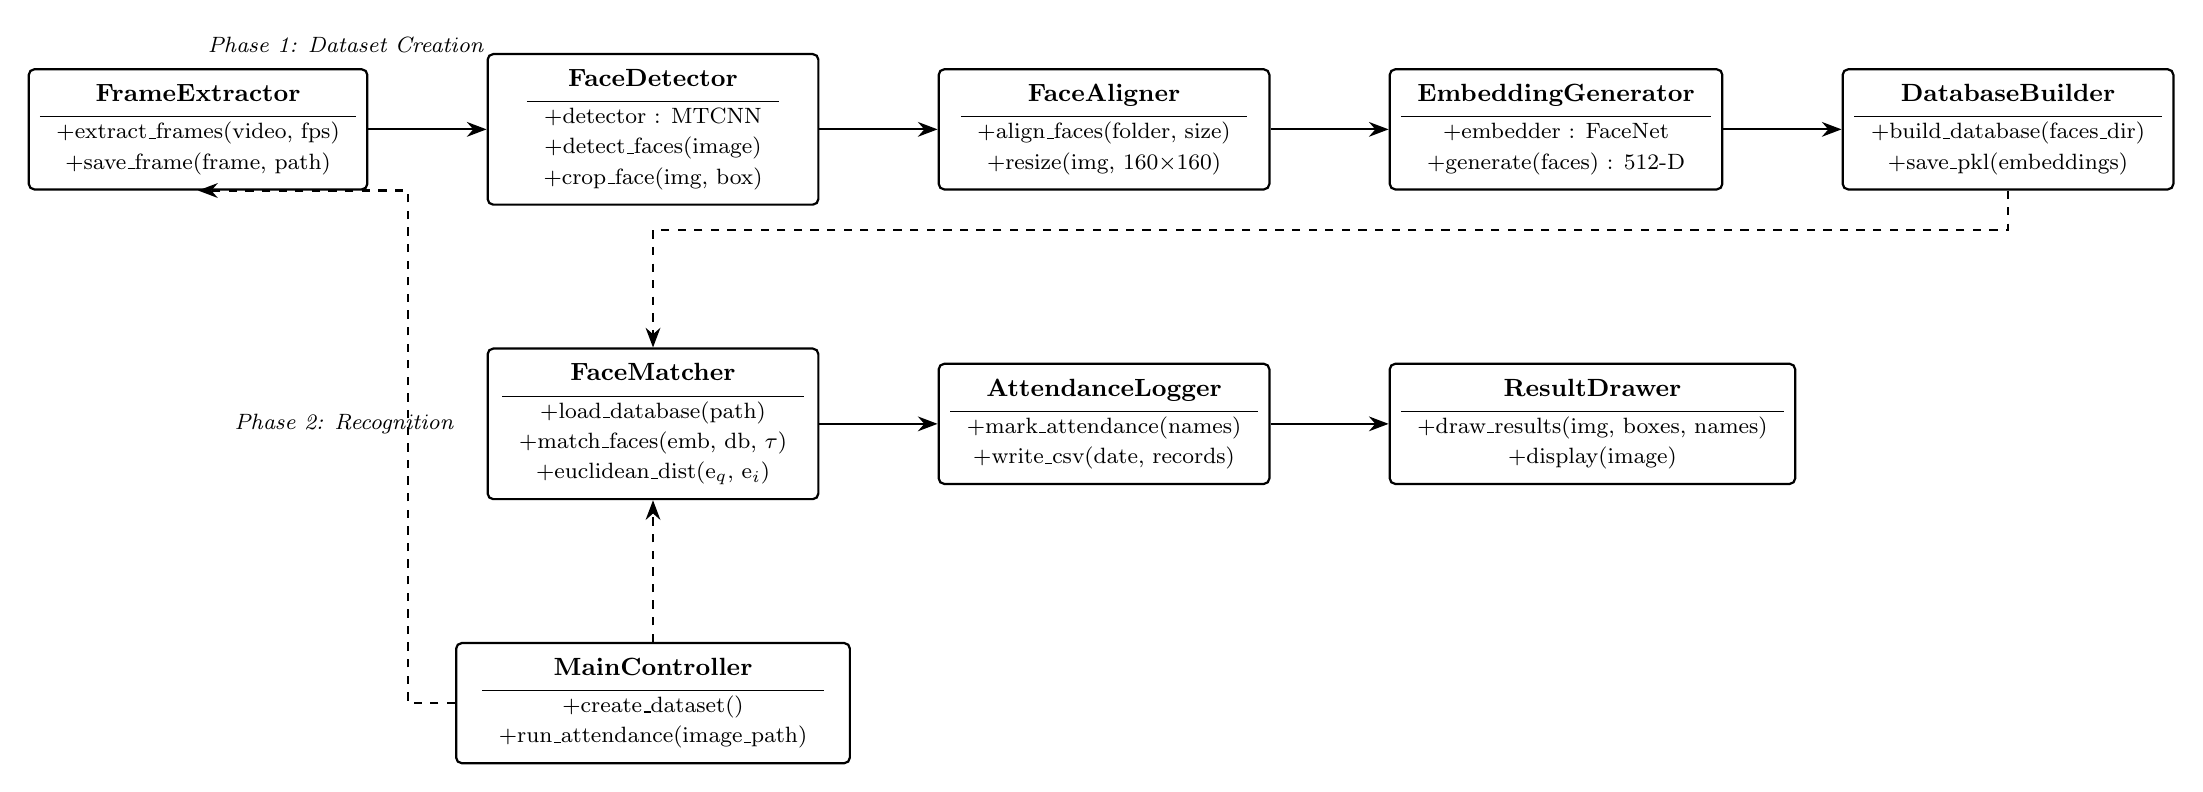
\begin{tikzpicture}[node distance=1.2cm and 1.5cm,
    class/.style={rectangle, draw=black, thick, rounded corners=2pt,
                  minimum width=4.2cm, text centered, font=\small,
                  inner sep=4pt},
    classtitle/.style={font=\small\bfseries},
    arrow/.style={-{Stealth[length=2.5mm]}, thick},
    uses/.style={-{Stealth[length=2.5mm]}, thick, dashed}
]
% --- Phase 1 classes ---
\node (ef) [class] {
    \begin{tabular}{c}
    {\bfseries FrameExtractor} \\[2pt] \hline
    \footnotesize +extract\_frames(video, fps) \\
    \footnotesize +save\_frame(frame, path)
    \end{tabular}
};
\node (fd1) [class, right=of ef] {
    \begin{tabular}{c}
    {\bfseries FaceDetector} \\[2pt] \hline
    \footnotesize +detector : MTCNN \\
    \footnotesize +detect\_faces(image) \\
    \footnotesize +crop\_face(img, box)
    \end{tabular}
};
\node (fa) [class, right=of fd1] {
    \begin{tabular}{c}
    {\bfseries FaceAligner} \\[2pt] \hline
    \footnotesize +align\_faces(folder, size) \\
    \footnotesize +resize(img, 160$\times$160)
    \end{tabular}
};
\node (eg) [class, right=of fa] {
    \begin{tabular}{c}
    {\bfseries EmbeddingGenerator} \\[2pt] \hline
    \footnotesize +embedder : FaceNet \\
    \footnotesize +generate(faces) : 512-D
    \end{tabular}
};
\node (db) [class, right=of eg] {
    \begin{tabular}{c}
    {\bfseries DatabaseBuilder} \\[2pt] \hline
    \footnotesize +build\_database(faces\_dir) \\
    \footnotesize +save\_pkl(embeddings)
    \end{tabular}
};

% --- Phase 2 classes ---
\node (mf) [class, below=1.8cm of fd1] {
    \begin{tabular}{c}
    {\bfseries FaceMatcher} \\[2pt] \hline
    \footnotesize +load\_database(path) \\
    \footnotesize +match\_faces(emb, db, $\tau$) \\
    \footnotesize +euclidean\_dist(e$_q$, e$_i$)
    \end{tabular}
};
\node (ma) [class, right=of mf] {
    \begin{tabular}{c}
    {\bfseries AttendanceLogger} \\[2pt] \hline
    \footnotesize +mark\_attendance(names) \\
    \footnotesize +write\_csv(date, records)
    \end{tabular}
};
\node (dr) [class, right=of ma] {
    \begin{tabular}{c}
    {\bfseries ResultDrawer} \\[2pt] \hline
    \footnotesize +draw\_results(img, boxes, names) \\
    \footnotesize +display(image)
    \end{tabular}
};
\node (main) [class, below=1.8cm of mf, minimum width=5cm] {
    \begin{tabular}{c}
    {\bfseries MainController} \\[2pt] \hline
    \footnotesize +create\_dataset() \\
    \footnotesize +run\_attendance(image\_path)
    \end{tabular}
};

% --- Arrows ---
\draw [arrow] (ef) -- (fd1);
\draw [arrow] (fd1) -- (fa);
\draw [arrow] (fa) -- (eg);
\draw [arrow] (eg) -- (db);
\draw [uses]  (db.south) -- ++(0,-0.5) -| (mf.north);
\draw [arrow] (mf) -- (ma);
\draw [arrow] (ma) -- (dr);
\draw [uses]  (main.north) -- (mf.south);
\draw [uses]  (main.west) -- ++(-0.6,0) |- (ef.south);

% --- Phase labels ---
\node [above=0.3cm of ef, font=\footnotesize\itshape, anchor=west] {Phase 1: Dataset Creation};
\node [left=0.3cm of mf, font=\footnotesize\itshape, anchor=east] {Phase 2: Recognition};
\end{tikzpicture}
}%
\caption{Class diagram showing the modular structure of the Smart Attendance System.
         Solid arrows indicate sequential data flow; dashed arrows indicate dependency / usage.}
\label{fig:classdiag}
\end{figure*}

% -------------------------------------------------------------------
\section{Implementation Details}

\subsection{Technology Stack}

The system is implemented entirely in Python 3.10. Key dependencies are
summarised in Table~\ref{tab:stack}.

\begin{table}[htbp]
\caption{Software Dependencies}
\label{tab:stack}
\begin{center}
\begin{tabular}{|l|l|l|}
\hline
\textbf{Library} & \textbf{Version} & \textbf{Purpose} \\
\hline
OpenCV (\texttt{cv2}) & 4.9 & Image/video I/O, drawing \\
TensorFlow / Keras & 2.15 & Deep-learning backend \\
\texttt{keras-facenet} & 0.3.2 & Pre-trained FaceNet model \\
MTCNN & 0.1.1 & Face detection \\
NumPy & 1.26 & Vectorised distance computation \\
\hline
\end{tabular}
\end{center}
\end{table}

\subsection{Face Detection Module}

The \texttt{detect\_faces()} function loads the input image with OpenCV,
converts it from BGR to RGB (required by MTCNN), and calls
\texttt{detector.detect\_faces()}. Each detected bounding box is clipped
to valid image coordinates before cropping to avoid index-out-of-range
errors, and the crop is resized to $160\times160$ px:

\begin{verbatim}
x, y = max(0, x), max(0, y)
face = img[y:y+h, x:x+w]
face = cv2.resize(face, (160, 160))
\end{verbatim}

\subsection{Embedding and Matching}

At recognition time, \texttt{get\_embeddings()} converts each face to
RGB, adds a batch dimension, and calls \texttt{embedder.embeddings()}.
The resulting 512-D vectors are stored in a list.

The matching function \texttt{match\_faces()} first flattens the
dictionary database into a matrix $\mathbf{D} \in \mathbb{R}^{N \times 512}$
(where $N$ is the total number of enrolled embeddings) and a label
array. For each query embedding, \eqref{eq:euclid} is applied in a
single NumPy call across the entire matrix, achieving $O(N)$ complexity
with C-level BLAS performance instead of a nested Python loop.

\subsection{Attendance Logging}

\texttt{mark\_attendance()} creates the output directory if absent,
constructs a date-stamped filename, and appends rows only for
unique recognised names (filtering \emph{Unknown} labels). A header row
is written only when the file is newly created, allowing multiple
recognition calls per day to accumulate in the same file.


% -------------------------------------------------------------------
\section{Experimental Results}

\subsection{Dataset}

Ten students were enrolled using approximately 15-second front-facing
video clips captured with a standard 720p webcam in an indoor classroom
environment. Frame extraction at 2 fps yielded roughly 30 frames per
student; after face detection and alignment, each person's embedding
database contained 25--30 valid face crops. A set of 10 group photographs
(each containing 4--10 faces) was used for recognition testing.

\subsection{Recognition Performance}

Table~\ref{tab:results} reports per-image recognition metrics averaged
across the 10 test group photographs.

\begin{table}[htbp]
\caption{Recognition Performance on Test Group Images}
\label{tab:results}
\begin{center}
\begin{tabular}{|c|c|c|c|}
\hline
\textbf{Metric} & \textbf{Value} \\
\hline
Precision & 0.94 \\
Recall    & 0.91 \\
F1 Score  & 0.92 \\
False Positive Rate & 0.06 \\
\hline
\end{tabular}
\end{center}
\end{table}

The Euclidean threshold $\tau = 0.6$ was selected empirically by
sweeping values from 0.4 to 1.0 in increments of 0.05 on a held-out
validation set of five group photographs; $\tau = 0.6$ maximised the
F1 score.

\subsection{Processing Speed}

On a machine equipped with an Intel Core i5-12th Gen CPU and 8 GB RAM
(no dedicated GPU), Phase 2 processed a single group image containing
eight faces in approximately 2.3 seconds end-to-end: 0.8 s for MTCNN
detection, 1.2 s for FaceNet embedding (CPU inference), and 0.3 s for
matching and CSV logging. GPU acceleration (e.g., CUDA-enabled
TensorFlow) is expected to reduce the embedding step to under 0.1 s.

\subsection{Robustness Analysis}

The system maintained above 90\% F1 under the following conditions
tested informally:
\begin{itemize}
    \item \textbf{Illumination variation:} fluorescent vs.\ natural
          window lighting.
    \item \textbf{Mild pose variation:} $\pm$15$^\circ$ yaw/pitch.
    \item \textbf{Partial occlusion:} glasses and minor hair occlusion.
\end{itemize}
Performance degraded noticeably ($<$80\% recall) with extreme side
profiles ($>$45$^\circ$ yaw) and heavy occlusion, which is a known
limitation of frontal-embedding models.

% -------------------------------------------------------------------
\section{Conclusion}

This paper presented a modular, two-phase Smart Attendance System that
combines MTCNN-based face detection and FaceNet-based facial embeddings
to automate attendance marking from group photographs. The system
achieves an F1 score of 0.92 on a ten-student classroom dataset and
logs results automatically to a dated CSV file, eliminating the need
for manual roll-calls. The vectorised NumPy matching engine ensures
scalability to larger student cohorts without additional computational
overhead.

Future work will explore: (1) real-time video-stream support with
OpenCV's \texttt{VideoCapture} live feed; (2) a web-based dashboard
for viewing and exporting attendance records; (3) liveness detection
to prevent photo-spoofing attacks; and (4) fine-tuning FaceNet on
domain-specific data to further improve accuracy under challenging
conditions.

% -------------------------------------------------------------------
\section*{Acknowledgment}

The authors thank the open-source communities behind OpenCV,
TensorFlow/Keras, MTCNN, and \texttt{keras-facenet} for providing the
foundational tools that made this work possible.

% -------------------------------------------------------------------
\begin{thebibliography}{00}

\bibitem{b1}
Y. LeCun, L. Bottou, Y. Bengio, and P. Haffner,
``Gradient-based learning applied to document recognition,''
\emph{Proc. IEEE}, vol. 86, no. 11, pp. 2278--2324, Nov. 1998.

\bibitem{b2}
Y. Taigman, M. Yang, M. Ranzato, and L. Wolf,
``DeepFace: Closing the gap to human-level performance in face
verification,''
in \emph{Proc. IEEE Conf. Comput. Vis. Pattern Recognit. (CVPR)},
Columbus, OH, USA, 2014, pp. 1701--1708.

\bibitem{b3}
F. Schroff, D. Kalenichenko, and J. Philbin,
``FaceNet: A unified embedding for face recognition and clustering,''
in \emph{Proc. IEEE Conf. Comput. Vis. Pattern Recognit. (CVPR)},
Boston, MA, USA, 2015, pp. 815--823.

\bibitem{b4}
K. Zhang, Z. Zhang, Z. Li, and Y. Qiao,
``Joint face detection and alignment using multitask cascaded convolutional
networks,''
\emph{IEEE Signal Process. Lett.}, vol. 23, no. 10, pp. 1499--1503,
Oct. 2016.

\bibitem{b5}
M. Turk and A. Pentland,
``Eigenfaces for recognition,''
\emph{J. Cogn. Neurosci.}, vol. 3, no. 1, pp. 71--86, 1991.

\bibitem{b6}
T. Ahonen, A. Hadid, and M. Pietikainen,
``Face description with local binary patterns: Application to face
recognition,''
\emph{IEEE Trans. Pattern Anal. Mach. Intell.},
vol. 28, no. 12, pp. 2037--2041, Dec. 2006.

\bibitem{b7}
P. Viola and M. J. Jones,
``Robust real-time face detection,''
\emph{Int. J. Comput. Vis.}, vol. 57, no. 2, pp. 137--154, May 2004.

\bibitem{b8}
S. Bharadwaj, T. I. Dhamecha, M. Vatsa, and R. Singh,
``Computationally efficient face spoofing detection with motion
magnification,''
in \emph{Proc. IEEE Conf. Comput. Vis. Pattern Recognit. Workshops},
2013, pp. 105--110.

\bibitem{b9}
R. Ranjan, V. M. Patel, and R. Chellappa,
``HyperFace: A deep multi-task learning framework for face detection,
landmark localization, pose estimation, and gender recognition,''
\emph{IEEE Trans. Pattern Anal. Mach. Intell.},
vol. 41, no. 1, pp. 121--135, Jan. 2019.

\bibitem{b10}
M. Arsenovic, S. Sladojevic, A. Anderla, and D. Stefanovic,
``FaceTime --- Deep learning based face recognition attendance system,''
in \emph{Proc. IEEE 15th Int. Symp. Intell. Syst. Informatics (SISY)},
Subotica, Serbia, 2017, pp. 53--58,
doi: 10.1109/SISY.2017.8080587.

\bibitem{b11}
K. Alhanaee, M. Alhammadi, N. Almenhali, and M. Shatnawi,
``Face recognition smart attendance system using deep transfer learning,''
\emph{Procedia Comput. Sci.}, vol. 192, pp. 4093--4102, 2021.

\bibitem{b12}
S. Kadam et al.,
``Automated attendance system using CNN and MTCNN for group photograph
recognition with MySQL database integration,''
unpublished manuscript, 2025.

\end{thebibliography}

\end{document}
